\title{
\centering

\includegraphics[width=4cm,height=4cm,keepaspectratio]{du.jpg} \\ \ CSE - 4255 Data Mining and Warehousing Lab\\  \Large \textit{Data Warehousing}\\}


\author{
        Saif Mahmud \\
        Roll: SH - 54\\
            \and
        M. Tanjid Hasan Tonmoy\\
        Roll: SH - 09\\
            \and
        \\\textbf{Submitted To:}\\ Dr. Chowdhury Farhan Ahmed \\
        Professor\\
        \\ \& \\ 
        Abu Ahmed Ferdaus\\
        Associate Professor\\ \\
        Department of Computer Science and Engineering\\
        University of Dhaka        
}
\date{\today}

\documentclass[12pt]{article}
\usepackage{graphicx}
\usepackage{cite}
\usepackage{url}
\usepackage{multirow}
\usepackage{longtable}
\usepackage{multirow}
\usepackage{subcaption}
%\usepackage[a4paper]{geometry}
\newcommand{\s}{\vspace{0.2cm}}
\usepackage{float}

\begin{document}


\maketitle
\thispagestyle{empty}
\clearpage
\newpage

\section{Problem Definition}
The tasks for this assignment is described below:
\begin{itemize}
	\item Creating a Relational Database
	\item Defining Schema (Star, Snowflake or Galaxy) for Data Warehouse
	\item Creating Dimension Table and Fact Table from Predefined Relational Database
	\item Creating Data Cuboid from Defined Schema
	\item OLAP operation on the data cube such as roll-up, drill-down etc.
\end{itemize}

\section{Theory}
A data warehouse is a subject-oriented, integrated, time-variant and nonvolatile collection of data in support of management’s decision making process. A data cube allows data to be modeled and viewed in multiple
dimensions. It is defined by dimensions and facts.

The most common modeling paradigm is the star schema, in which the data warehouse contains (1) a large central table (fact table) containing the bulk of the data, with no redundancy, and (2) a set of smaller attendant tables (dimension tables), one for each dimension. The schema graph resembles a starburst, with the dimension tables displayed in a radial pattern around the central fact table.

The snowflake schema is a variant of the star schema model, where some dimension tables are normalized, thereby further splitting the data into additional tables. The resulting schema graph forms a shape similar to a snowflake.

Sophisticated applications may require multiple fact tables to share dimension tables. This kind of schema can be viewed as a collection of stars, and hence is called a galaxy schema or a fact constellation.

The roll-up operation (also called the drill-up operation by some vendors)
performs aggregation on a data cube, either by climbing up a concept hierarchy for a dimension or by dimension reduction.

Drill-down is the reverse of roll-up. It navigates from less detailed data to more detailed data. Drill-down can be realized by either stepping down a concept hierarchy for a dimension or introducing additional dimensions.

\section{Experiment Setup}
\subsection{Schema}
We designed a star schema simulating warehousing on relational a retail database. The schema is illustrated in 

\begin{figure}[H]
	\centering
	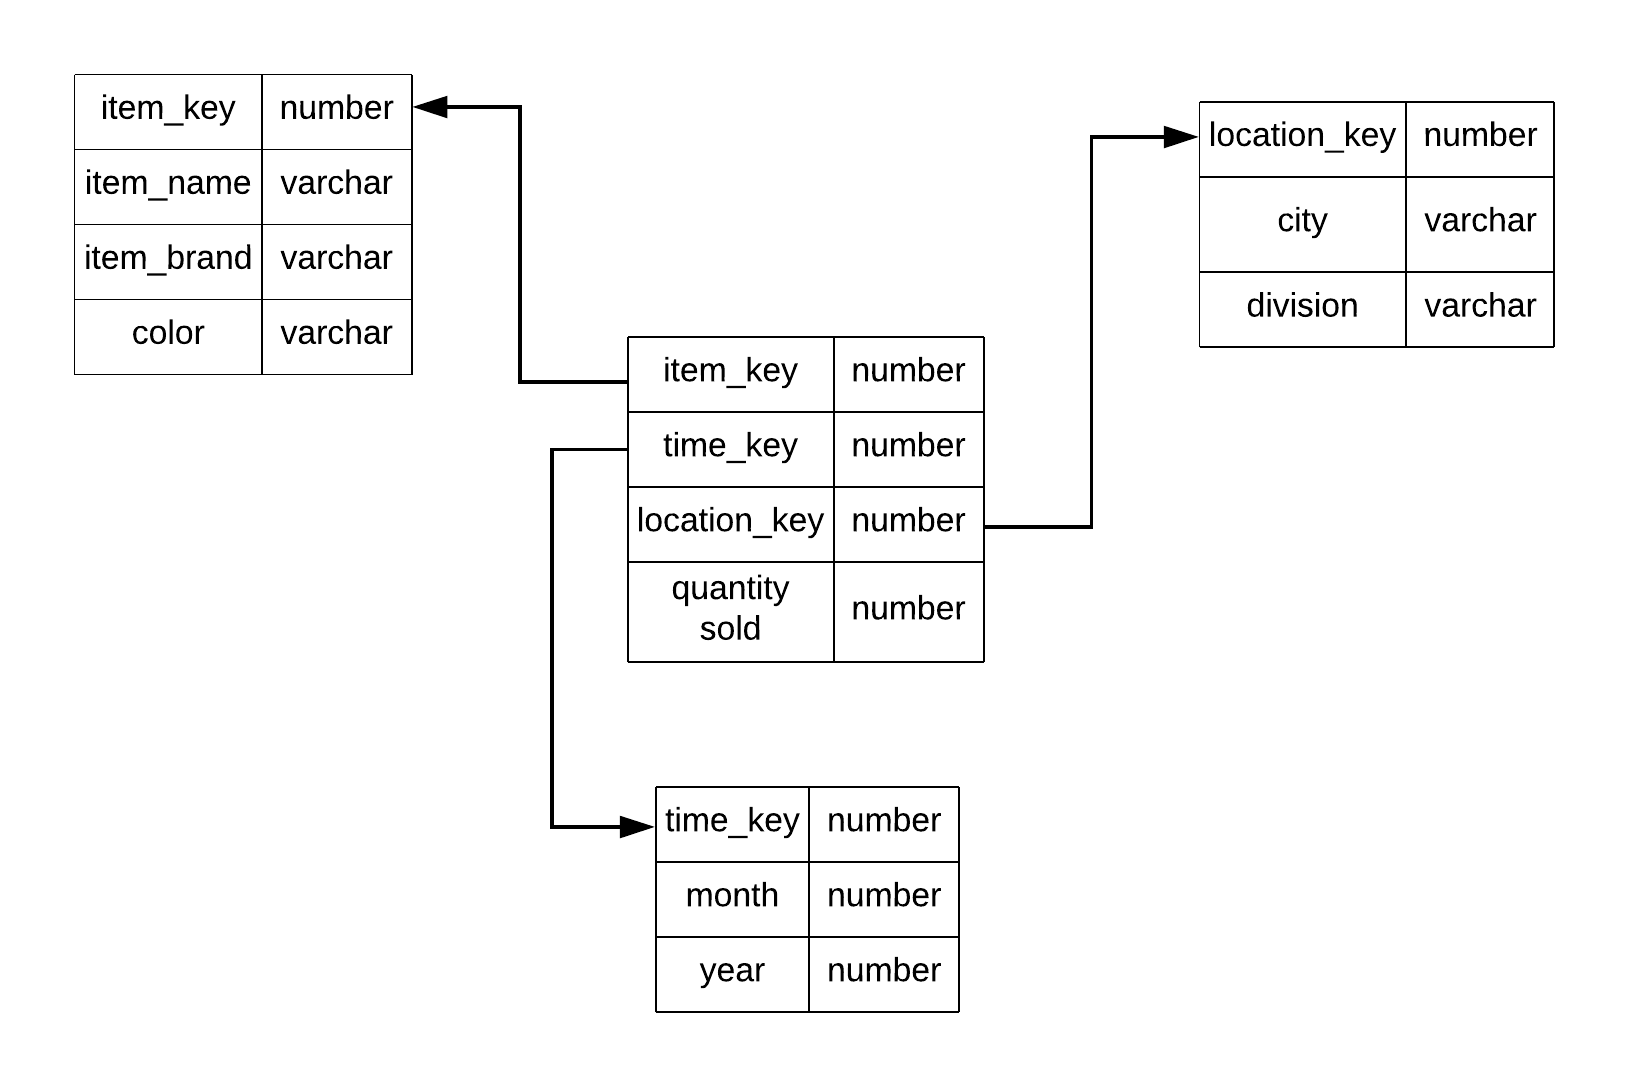
\includegraphics[]{schema.png}
	\caption{Star Schema used in the experiment}
\end{figure}

\subsection{Operations}
We have implemented Relational OLAP using oracle database. The operations are as follows 

\subsubsection*{Roll up}
\begin{figure}[H]
	\centering
	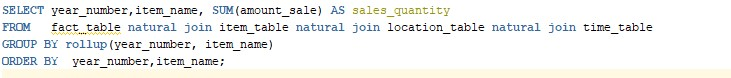
\includegraphics[]{rollup-code.jpg}
\end{figure}
\begin{figure}[h!]
	\centering
	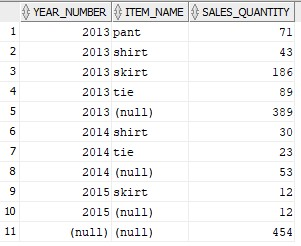
\includegraphics[]{rollup.jpg}
	\caption{Rollup grouping output}
\end{figure}

\subsubsection*{Cube}

\begin{figure}[h!]
	\centering
	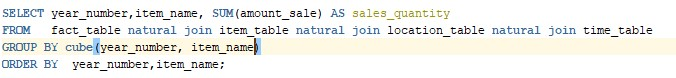
\includegraphics[]{cube-code.jpg}
\end{figure}

\begin{figure}[H]
	\centering
	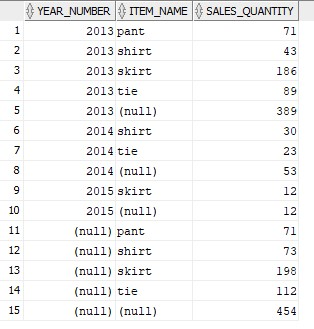
\includegraphics[]{cube.jpg}
	\caption{Cube grouping output}
\end{figure}
\subsubsection*{Slice and Dice}
\begin{figure}[H]
	\centering
	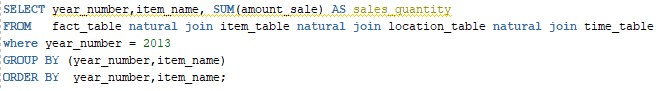
\includegraphics[]{sd-code.jpg}
\end{figure}

\begin{figure}[H]
	\centering
	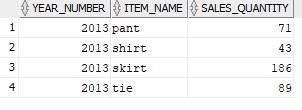
\includegraphics[]{sd.jpg}
	\caption{Slicing output}
\end{figure}
\section{Conclusion}
The separation of operational databases from data warehouses is based on
the different structures, contents, and uses of the data in these two systems. Decision support requires historic data, whereas operational databases do not typically maintain historic data. In this context, the data in operational databases, though abundant, are
usually far from complete for decision making. Decision support requires consolidation
(e.g., aggregation and summarization) of data from heterogeneous sources, resulting
in high-quality, clean, integrated data. In contrast, operational databases contain only
detailed raw data, such as transactions, which need to be consolidated before analysis.
Because the two systems provide quite different functionalities and require different
kinds of data, it is presently necessary to maintain separate databases. Decision
Data warehouse assists the decision making process by providing a historical perspective based on need. We have simulated such operations in a synthetic retail data warehouse.


\end{document}
